\section{Objective-Specific Checks}
\label{app:results-details}
\subsection{O1: Partial ownership and regression robustness}
\label{app:results-o1}
\begin{mergedcontribution}{authorSowmya}
\subsubsection{Measures and model}
\label{app:o1-definitions}
\label{app:o1-dictionary}
The grouping adjustment is Ownership-HHI minus Brand-HHI, and the partial-ownership adjustment is MHHI minus Ownership-HHI. Their sum is MHHI minus Brand-HHI. The IndiGo ratio divides its share by the second-largest group's share.

\label{app:review-o1-formulae}
MHHI adds a partial-ownership adjustment to the common index in Appendix~\ref{app:shared-calculations}:
\begin{equation}
\text{MHHI}_t = \text{Ownership-HHI}_t+\sum_{j}\sum_{k\neq j}\lambda_{jk}S_{jt}S_{kt},\qquad
\lambda_{jk}=\frac{\sum_i \gamma_{ij}\beta_{ik}}{\sum_i \gamma_{ij}\beta_{ij}} \tag{O1.1b}\label{eq:review-o1-mhhi}
\end{equation}
Here $\beta_{ik}$ is owner $i$'s stake in firm $k$ and $\gamma_{ik}$ its control share \parencite{obriensalop2000}. The regression is
\begin{equation}
\text{Index}_t = \alpha + \beta t + \sum_{k=1}^{4}\gamma_k\,\text{Post}_{kt} + \delta\,\text{COVID}_t + \sum_{m=2}^{12}\mu_m M_{mt} + \varepsilon_t \tag{O1.2}\label{eq:review-o1-regression}
\end{equation}
Here $\beta$ is the monthly trend, $\gamma_k$ the four permanent event steps, $\delta$ the COVID effect and $\mu_m$ the seasonal effects (January base). Dates and controls follow Section~\ref{sec:method-o1}. Standard errors follow \textcite{neweywest1987}.
\begin{samepage}
For each of Brand HHI, Ownership HHI and MHHI, let $x_t$ be the change from the previous available observation. The modified score is
\begingroup
\renewcommand{\theHequation}{review-o1-jump}
\begin{equation}
M_t=\frac{0.6745\,[x_t-\operatorname{median}(x)]}{\operatorname{median}|x-\operatorname{median}(x)|}.
\tag{O1.3}\label{eq:review-o1-jump}
\end{equation}
\endgroup
\par\end{samepage}
The median and MAD use all observed changes \parencite{iglewicz1993outliers}. Missing April 2020 makes May's change span March--May. Apply the flag and nearby-window rules in Section~\ref{sec:method-o1}; the pass/fail outcomes are reported with Table~\ref{tab:o1-drift}.


\subsubsection{Period summaries}
\label{app:eda-national-inputs}

\begin{minipage}{\linewidth}
\captionsetup{font={small,color=authorSowmya},labelfont=bf,justification=raggedright,singlelinecheck=false,hypcap=false}
\captionof{table}{O1: Concentration measures by period (period means).}
\label{tab:o1-periods}
\centering
{\small\setstretch{1.1}\setlength{\tabcolsep}{4pt}
\fontsize{10}{12}\selectfont\setstretch{1}\setlength{\tabcolsep}{3pt}
\renewcommand{\arraystretch}{1.15}
\begin{tabular}{|>{\raggedright\arraybackslash}p{\dimexpr0.28\linewidth-2\tabcolsep-1.1428571428571428\arrayrulewidth\relax}|>{\raggedright\arraybackslash}p{\dimexpr0.12\linewidth-2\tabcolsep-1.1428571428571428\arrayrulewidth\relax}|>{\raggedright\arraybackslash}p{\dimexpr0.12\linewidth-2\tabcolsep-1.1428571428571428\arrayrulewidth\relax}|>{\raggedright\arraybackslash}p{\dimexpr0.12\linewidth-2\tabcolsep-1.1428571428571428\arrayrulewidth\relax}|>{\raggedright\arraybackslash}p{\dimexpr0.12\linewidth-2\tabcolsep-1.1428571428571428\arrayrulewidth\relax}|>{\raggedright\arraybackslash}p{\dimexpr0.12\linewidth-2\tabcolsep-1.1428571428571428\arrayrulewidth\relax}|>{\raggedright\arraybackslash}p{\dimexpr0.12\linewidth-2\tabcolsep-1.1428571428571428\arrayrulewidth\relax}|}
\hline
\textbf{Period} & \textbf{Brand HHI} & \textbf{Own.\ HHI} & \textbf{MHHI} & \textbf{CR2 (\%)} & \textbf{Gap (pp)} & \textbf{Fringe (\%)} \\
\hline
Pre-Jet exit (Jan 2015--Apr 2019) & 2{,}323.8 & 2{,}408.0 & 2{,}416.1 & 58.7 & 21.8 & 41.3 \\
\hline
Jet exit to Tata (May 2019--Dec 2021) & 3{,}293.1 & 3{,}294.5 & 3{,}342.3 & 66.9 & 39.2 & 33.1 \\
\hline
Tata to mergers (Jan 2022--Nov 2024) & 3{,}847.6 & 4{,}308.6 & 4{,}308.6 & 85.5 & 33.1 & 14.5 \\
\hline
Post mergers (Dec 2024--Jul 2026) & 4{,}538.0 & 4{,}876.7 & 4{,}876.7 & 90.7 & 38.0 & 9.3 \\
\hline
\end{tabular}\par}
\vspace{4pt}
{\footnotesize\setstretch{1.1}\raggedright\textit{Note:} HHI values are index points; CR2, gap and fringe use ownership-group passenger shares. April 2020 is missing and not imputed.\par
\textit{Source:} DGCA monthly airline traffic via \href{https://github.com/mkubicek/india-aviation-stats/tree/16770ac59dae61ce7b80fd8bd67dd7f4cef280a6}{Kubicek (2026)}; authors' calculations.\par}
\end{minipage}

\subsubsection{Ownership inputs and sensitivity}
\label{app:o1-stakes}
Apply the stakes in Table~\ref{tab:o1-stakes} to Equation~\ref{eq:review-o1-mhhi}. Proportional control sets $\gamma_{ik}=\beta_{ik}$. The alternative assigns full control to the majority owner. Firms without listed stakes are treated as wholly owned.

\begin{minipage}{\linewidth}
\captionsetup{font={small,color=authorSowmya},labelfont=bf,justification=raggedright,singlelinecheck=false,hypcap=false}
\captionof{table}{O1: Partial-ownership schedule used for MHHI (financial stakes $\beta$).}
\label{tab:o1-stakes}
\centering
{\footnotesize\setstretch{1.0}\setlength{\tabcolsep}{4pt}
\fontsize{10}{12}\selectfont\setstretch{1}\setlength{\tabcolsep}{3pt}
\renewcommand{\arraystretch}{1.15}
\begin{tabular}{|l|l|r|r|r|c|}
\hline
\textbf{Firm} & \textbf{Months applied} & \textbf{Tata} & \textbf{Partner} & \textbf{Other} & \textbf{Source} \\
\hline
Vistara & Jan 2015--Dec 2021 & 51 & 49 & -- & a \\
\hline
AirAsia India & Jan--Aug 2015 & 30 & 49 & 21 & b \\
\hline
AirAsia India & Sep 2015--Mar 2016 & 41.06 & 49 & 9.94 & c \\
\hline
AirAsia India & Apr 2016--Dec 2019 & 49 & 49 & 2 & c, d \\
\hline
AirAsia India & Jan--Dec 2020 & 51 & 49 & -- & e \\
\hline
AirAsia India & Jan--Dec 2021 & 83.67 & 16.33 & -- & e, f \\
\hline
\end{tabular}\par}
\vspace{4pt}
{\footnotesize\setstretch{1.0}\raggedright
\textit{Note:} Partner means Singapore Airlines for Vistara and AirAsia Investment for AirAsia India. Other means Telestra through March 2016, then two individuals. Stakes apply from the month after the announcement. The undated increase to 51\% is assigned to January 2020. Assigning April 2016 instead changes the mean adjustment from 22.9 to 23.1 points. Foreign partners hold no other Indian airline stake and enter only $\lambda$'s denominator.\par
\textit{Sources:} (a) \textcite{sia2015annual,sia2022merger}; (b) \textcite{airasia2013jv}; (c) \textcite{tata2016airasia}; (d) \textcite{airasia2018q4}; (e) \textcite{airasia2021disposal}; (f) \textcite{airasia2021results}. Stakes are percentages; dashes indicate no other stake.\par}
\end{minipage}

Interpolating the 2017 gap raises the pre-2022 mean adjustment from 22.9 to 24.9 points. Full control of Vistara gives a mean of 36.9 and maximum of 119.6 points.

\subsubsection{Data and regression checks}
\label{app:o1-cleaning}
Table~\ref{tab:o1-cleansing} gives the cleaning totals. There are no missing key fields or duplicate airline-months. The January 2024 AIX Connect rebrand is retained. Two positive-passenger records have zero ASK/RPK (Air Odisha, September 2018, and Air Deccan, March 2020) and remain flagged.

Of the outlier flags, 45 are COVID/market-wide, 23 entry/exit, one merger and 23 unexplained with less than 1\% share. Dropping the last group changes Brand-HHI by at most 70.6 points and Ownership-HHI/MHHI by 34.5. Of 12 within-spell missing runs, AirAsia India's January--December 2017 gap is material (bracketing share 3.6\%, HHI overstatement about 165--171 points). Only sensitivity runs interpolate it. Go First's May 2020 lockdown suspension is not imputed.


\label{app:o1-cr2}
\label{app:o1-robust}
Re-dating Jet and Go First steps to the drifts gives Ownership-HHI steps 396, 933, 696 and 186 (sum 2,211; $R^2=0.985$); Brand-HHI and MHHI sums are 1,801 and 2,162, all steps significant at 1\%.

\begin{minipage}{\linewidth}
\captionsetup{font={small,color=authorSowmya},labelfont=bf,justification=raggedright,singlelinecheck=false,hypcap=false}
\captionof{table}{O1: Ownership-HHI robustness and CR2 event checks.}
\label{tab:o1-robust}
\label{tab:o1-cr2reg}
\label{tab:detail-o1-regression}
\centering
{\small\setstretch{1.1}\setlength{\tabcolsep}{5pt}
\fontsize{10}{12}\selectfont\setstretch{1}\setlength{\tabcolsep}{3pt}
\renewcommand{\arraystretch}{1.15}
\begin{tabular}{|>{\raggedright\arraybackslash}p{\dimexpr0.44\linewidth-2\tabcolsep-1.2\arrayrulewidth\relax}|>{\raggedright\arraybackslash}p{\dimexpr0.14\linewidth-2\tabcolsep-1.2\arrayrulewidth\relax}|>{\raggedright\arraybackslash}p{\dimexpr0.14\linewidth-2\tabcolsep-1.2\arrayrulewidth\relax}|>{\raggedright\arraybackslash}p{\dimexpr0.14\linewidth-2\tabcolsep-1.2\arrayrulewidth\relax}|>{\raggedright\arraybackslash}p{\dimexpr0.14\linewidth-2\tabcolsep-1.2\arrayrulewidth\relax}|}
\hline
\textbf{Specification} & \textbf{Jet exit} & \textbf{Tata} & \textbf{Go First} & \textbf{Mergers} \\
\hline
Baseline (Newey--West 12 lags) & 312 (3.9) & 900 (10.8) & 640 (11.4) & 137 (2.5) \\
\hline
Newey--West 6 lags & 312 (3.8) & 900 (9.8) & 640 (10.4) & 137 (2.2) \\
\hline
Newey--West 18 lags & 312 (4.6) & 900 (12.1) & 640 (12.0) & 137 (2.8) \\
\hline
COVID months dropped & 330 (4.6) & 899 (10.6) & 656 (12.0) & 136 (2.5) \\
\hline
AirAsia India 2017 interpolated & 371 (4.0) & 920 (10.0) & 652 (10.6) & 148 (2.6) \\
\hline
\multicolumn{5}{|l|}{CR2 event steps in pp, with Newey--West (12-lag) standard errors} \\
\hline
Ownership-group CR2 & 5.72 (0.95) & 17.95 (1.18) & 9.29 (1.31) & 1.41 (0.58) \\
\hline
Brand CR2 & 6.95 (1.07) & 1.90 (0.92) & 6.47 (0.76) & 6.53 (0.74) \\
\hline
\end{tabular}\par}
\par\vspace{4pt}
{\fontsize{10}{12}\selectfont\setstretch{1}\setlength{\tabcolsep}{3pt}
\renewcommand{\arraystretch}{1.15}
\begin{tabular}{|>{\raggedright\arraybackslash}p{\dimexpr0.24\linewidth-2\tabcolsep-1.2\arrayrulewidth\relax}|*{4}{>{\centering\arraybackslash}p{\dimexpr0.19\linewidth-2\tabcolsep-1.2\arrayrulewidth\relax}|}}
\hline
\textbf{CR2 series} & \textbf{Step sum} & \textbf{Trend} & \textbf{COVID} & \textbf{$R^2$ / DW}\\
\hline
Ownership & 34.4 (2.6) & $-0.02$ (0.02) & 5.03 (0.73) & 0.984 / 0.80\\
\hline
Brand & 21.9 (2.8) & 0.01 (0.03) & 4.44 (0.77) & 0.958 / 0.84\\
\hline
\end{tabular}\par}
{\footnotesize\raggedright HHI parentheses contain $t$-statistics. CR2 parentheses contain Newey--West standard errors (12 lags). HHI residual Durbin--Watson values are 0.92, 0.93 and 0.94 for Brand, Ownership and MHHI. In all five models, Breusch--Godfrey (12 lags) rejects no autocorrelation and ADF rejects a residual unit root ($p<0.001$). Source: authors' calculations.\par}
\end{minipage}
\vspace{0.8em}

\subsubsection{Model fit and observed changes}
\begin{minipage}{\linewidth}
\centering
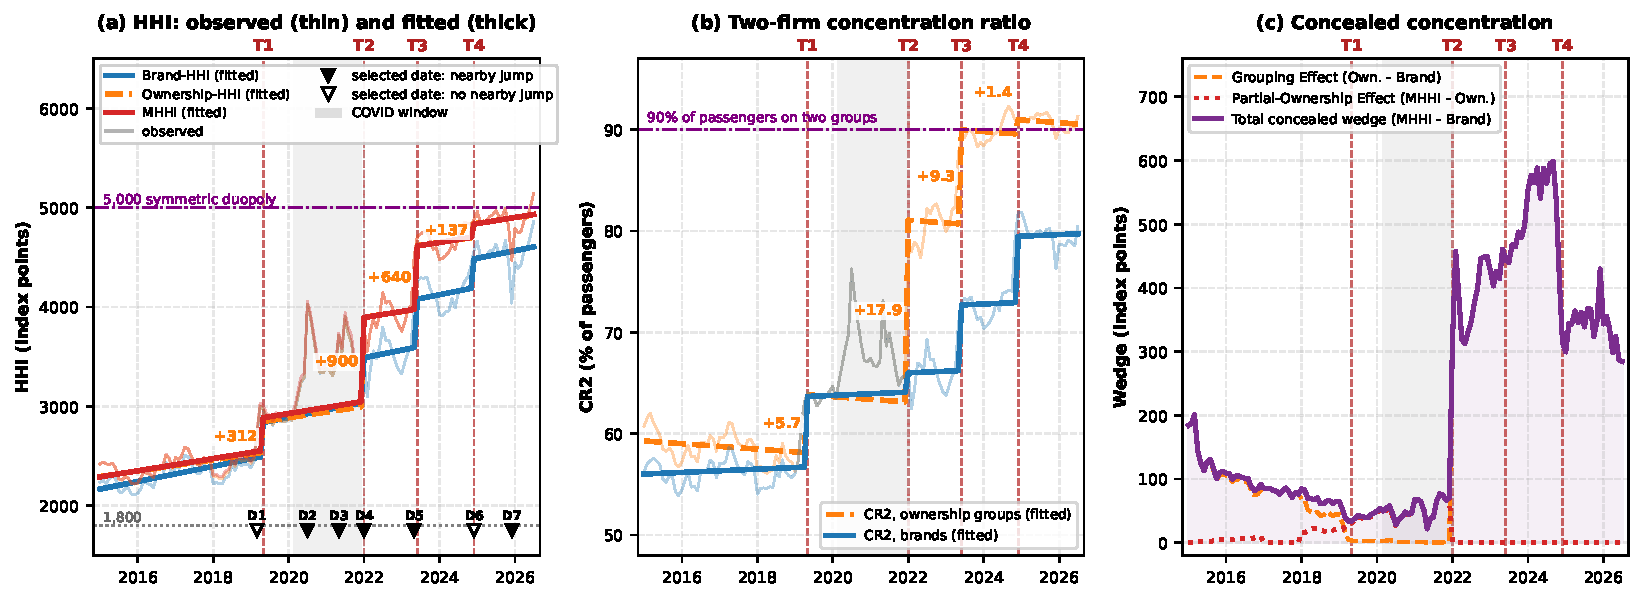
\includegraphics[width=\linewidth]{review/shortening/figures/o1_indices_review.pdf}
\captionof{figure}{O1: Interrupted time-series view of national concentration, January 2015--July 2026.}
\label{fig:o1-its}
\vspace{2pt}
\par\footnotesize\setstretch{1.1}
\textit{Note:} Thin/thick lines show observed/fitted series after netting out COVID and seasonality. Panels show (a) HHI series, (b) CR2 and (c) grouping, partial-ownership and total adjustments. Step labels give Ownership-HHI points in (a) and CR2 percentage points in (b). T1--T4 mark Jet's exit, Tata's acquisition, Go First's exit and the legal mergers. D1--D7 are the windows in Table~\ref{tab:o1-drift}. Filled markers have a jump within 40 days; hollow markers do not. Grey shading marks COVID.\par
\textit{Source:} DGCA monthly traffic via \href{https://github.com/mkubicek/india-aviation-stats/tree/16770ac59dae61ce7b80fd8bd67dd7f4cef280a6}{Kubicek (2026)}; authors' calculations.
\end{minipage}

\Needspace{4\baselineskip}


\par
\begingroup
\flowtablestyle
\fontsize{10}{12}\selectfont
\begin{longtable}{|>{\raggedright\arraybackslash}p{\dimexpr0.06\linewidth-2\tabcolsep-1.25\arrayrulewidth\relax}|>{\raggedright\arraybackslash}p{\dimexpr0.19\linewidth-2\tabcolsep-1.25\arrayrulewidth\relax}|>{\raggedright\arraybackslash}p{\dimexpr0.45\linewidth-2\tabcolsep-1.25\arrayrulewidth\relax}|>{\raggedright\arraybackslash}p{\dimexpr0.3\linewidth-2\tabcolsep-1.25\arrayrulewidth\relax}|}
\caption{Share movements and coincident events for the windows in Table~\ref{tab:o1-drift}.}\label{tab:detail-o1-drift}\\
\hline
\textbf{ID} & \textbf{Window} & \textbf{Largest share movements (pp)} & \textbf{Coincident event}\\
\hline
\endfirsthead
\multicolumn{4}{c}{Table~\thetable\ (continued)}\\
\hline
\textbf{ID} & \textbf{Window} & \textbf{Largest share movements (pp)} & \textbf{Coincident event}\\
\hline
\endhead
\endfoot
\endlastfoot
D1 & Feb--Apr 2019 & Jet group $-10.4$; IndiGo $+6.4$ & Jet Airways exit\\
\hline
D2 & Jun--Jul 2020 & IndiGo $+7.6$; Air India Group $-3.3$ & Restart after the COVID lockdown\\
\hline
D3 & Apr--May 2021 & Air India Group $+6.1$; AirAsia India $-3.2$ & Second COVID wave\\
\hline
D4 & Dec 2021--Jan 2022 & Air India Group $+13.9$ (Vistara $-7.7$, AirAsia India $-6.3$) & Tata acquisition and ownership regrouping\\
\hline
D5 & Apr--Jun 2023 & Go First $-6.4$; IndiGo $+5.7$ & Go First exit\\
\hline
D6 & Nov--Dec 2024 & Vistara, AIX Connect folded into Air India, Air India Express & AIX Connect and Vistara legal mergers\\
\hline
D7 & Nov--Dec 2025 & IndiGo $-4.0$; Air India Group $+2.8$ & IndiGo operational disruption \parencite{moca2026indigo}\\*
\noalign{\hrule height\arrayrulewidth\nobreak}
\multicolumn{4}{@{}p{\linewidth}@{}}{\resultstablenotes{Coincident events provide context, not causal estimates.}{DGCA monthly traffic via Kubicek (2026), ownership records and the cited regulatory release.}}\\
\end{longtable}
\endgroup


\Needspace{4\baselineskip}


\label{app:o1-wedge}

\begin{minipage}{\linewidth}
\captionsetup{font={small,color=authorSowmya},labelfont=bf,justification=raggedright,singlelinecheck=false,hypcap=false}
\captionof{table}{O1: Grouping-gap regression checks (Ownership-HHI minus Brand-HHI).}
\label{tab:o1-gap}
\centering
{\small\setstretch{1.1}\setlength{\tabcolsep}{5pt}
\fontsize{10}{12}\selectfont\setstretch{1}\setlength{\tabcolsep}{3pt}
\renewcommand{\arraystretch}{1.15}
\begin{tabular}{|l|r|r|}
\hline
\textbf{Coefficient} & \textbf{Standard model} & \textbf{With post-Tata trend} \\
\hline
Post-Tata step & 450.48\textsuperscript{**} (25.58) & 427.96\textsuperscript{**} (18.97) \\
\hline
Post-Tata trend (points/month) & -- & 5.52\textsuperscript{**} (1.95) \\
\hline
Post-Go First step & 158.05\textsuperscript{**} (38.93) & 72.18 (40.93) \\
\hline
Post-legal mergers step & $-153.84$\textsuperscript{**} (28.98) & $-247.66$\textsuperscript{**} (38.79) \\
\hline
$R^2$ & 0.968 & 0.976 \\
\hline
\end{tabular}\par}
\vspace{4pt}
{\footnotesize\setstretch{1.1}\raggedright\textit{Note:} Newey--West standard errors (12 lags) are in parentheses. \textsuperscript{**}$p<0.01$. Models include trend, COVID and month indicators. The Jet step is not significant. Source: authors' calculations.\par}
\end{minipage}

\end{mergedcontribution}

\subsection{O2: Exit absorption and fixed-share consolidation}
\label{app:results-o2}
\begin{mergedcontribution}{authorMeena}
\subsubsection{Inputs and formulas}
\label{app:o2-definitions}
For exiting group $e$, survivor $g$ and equally weighted window-average shares from Appendix~\ref{app:shared-calculations},
\[
a_g=100\frac{\bar s_{g,\mathrm{post}}-\bar s_{g,\mathrm{pre}}}{\bar s_{e,\mathrm{pre}}},\qquad
c_g=\bar s_{g,\mathrm{post}}^2-\bar s_{g,\mathrm{pre}}^2,\qquad
\Delta\HHI=\sum_g c_g.
\]
Apply these formulas separately to passenger and ASK shares. Include the exiting group's contribution when summing $c_g$. Windows are specified in Table~\ref{tab:o2-absorption}.

\begin{table}[H]
\centering
\color{authorMeena}
\caption{O2: Fixed Tata shares and exit-window market inputs.}\label{tab:o2-tata}\label{tab:o2-market}
\fontsize{10}{12}\selectfont\setstretch{1}\setlength{\tabcolsep}{3pt}
\renewcommand{\arraystretch}{1.15}
\begin{tabular}{|l|r|r|r|r|r|}
\hline
\multicolumn{6}{|l|}{Panel A: Pre-consolidation passenger shares (\%)}\\
\hline
\textbf{Step (share month)} & \textbf{Air India} & \textbf{AI Express} & \textbf{Vistara} & \textbf{AirAsia/AIX} & \textbf{Total}\\
\hline
Jan 2022 (Dec 2021) & 8.39 & 0.07 & 7.72 & 6.28 & 22.46\\
\hline
Dec 2024 (Sep 2024) & 11.14 & 3.97 & 10.04 & 4.11 & 29.26\\
\hline
\multicolumn{6}{|l|}{Panel B: Monthly averages around exits}\\
\hline
\textbf{Exit: window} & \textbf{Pax (m)} & \textbf{ASK (bn)} & \textbf{PLF (\%)} & \multicolumn{2}{r|}{\textbf{Groups $\geq1\%$}}\\
\hline
Jet: Apr 2018--Mar 2019 & 11.69 & 13.07 & 86.0 & \multicolumn{2}{r|}{8.0}\\
\hline
Jet: May 2019--Feb 2020 & 12.25 & 13.60 & 87.1 & \multicolumn{2}{r|}{7.0}\\
\hline
Go: May 2022--Apr 2023 & 11.53 & 13.29 & 84.1 & \multicolumn{2}{r|}{5.6}\\
\hline
Go: Jun 2023--May 2024 & 12.88 & 14.25 & 87.2 & \multicolumn{2}{r|}{4.6}\\
\hline
\end{tabular}
\sourcenote{DGCA via \textcite{kubicek2026aviationstats}; authors' calculations. AirAsia India was renamed AIX Connect. September 2024 precedes its October merger and Vistara's November merger. Pax: million passengers; ASK: billion seat-km; PLF $=100\mathrm{RPK}/\mathrm{ASK}$. Group count is the monthly average number with at least 1\% passenger share.}
\end{table}

\subsubsection{Worked exit and consolidation examples}
\label{app:workings}
\textbf{Exit check.} Jet's pre-exit mean share is 13.82\%; IndiGo moves from 42.78\% to 47.99\%. Substitution gives
\[
\begin{aligned}
\Delta\bar s_I&=47.99-42.78=5.21\ \mathrm{pp}, &
a_I&=100(5.21/13.82)\approx37.7\%,\\
c_I&=47.99^2-42.78^2\approx473, &
c_{\mathrm{Jet}}&=0^2-13.82^2\approx-191.
\end{aligned}
\]
Summing the unrounded contributions gives $+444$ points (Table~\ref{tab:detail-o2-absorption}), using HHI of period-average shares, not average monthly HHI.

\textbf{Fixed-share acquisition, January 2022.} December 2021 shares in Table~\ref{tab:o2-tata} give Air India plus Air India Express 8.46\%, Vistara 7.72\% and AirAsia India 6.28\%. Holding every share fixed,
\[
\begin{aligned}
\Delta\HHI_{\mathrm{mechanical}}
&=(8.46+7.72+6.28)^2-(8.46^2+7.72^2+6.28^2)\\
&=2(8.46\times7.72+8.46\times6.28+7.72\times6.28)\approx334.
\end{aligned}
\]
Observed change, January--December 2021 versus January--December 2022: 373 points. Difference: $373-334=39$ points.

\textbf{Late-2024 mergers.} Use September 2024 brand shares from Table~\ref{tab:o2-tata} and calculate the two merger pairs separately:
\[
\begin{aligned}
\Delta\HHI_{\text{AI--Vistara}} &= 2(11.14)(10.04) \approx 223.7,\\
\Delta\HHI_{\text{AI Express--AIX Connect}} &= 2(3.97)(4.11) \approx 32.6,\\
\Delta\HHI_{\text{total}} &\approx 223.7+32.6 \approx 256\text{ points}.
\end{aligned}
\]
Both merger pairs contribute to the 256-point total. The observed change between October 2023--September 2024 and December 2024--November 2025 is 493 points. Difference: $493-256=237$ points. A separate squared-average-share breakdown gives Tata brands $+135$, IndiGo $+380$, SpiceJet $-12$ and Akasa Air $+5$; it is not an exact decomposition of the 493-point average-monthly-HHI change.

\textbf{Effective firms and illustrative markups.} Reciprocals of the rounded mean monthly ownership HHIs give Jet $10{,}000/2{,}440=4.1\to10{,}000/2{,}870=3.5$ and Go First $10{,}000/3{,}940=2.5\to10{,}000/4{,}620=2.2$ (approximately). Cournot's share-weighted markup fraction is $\bar L=(\HHI/10{,}000)/|\varepsilon|$. Assuming fixed $|\varepsilon|=1.5$, the exit decompositions give $100\Delta\bar L=444/(100\times1.5)=2.96$ pp and $690/(100\times1.5)=4.60$ pp. These use HHI of average shares, unlike the effective-firm inputs; neither elasticity nor fare effects are estimated.

\subsubsection{Group results and source records}

\par
\begingroup
\flowtablestyle
\small
\setlength{\tabcolsep}{5pt}
\renewcommand{\arraystretch}{1.15}
\begin{longtable}{|l|r|r|r|r|r|r|}
\caption{Share of the exiting airline absorbed by each group, and contribution to the change in \HHI{}}\label{tab:detail-o2-absorption}\\
\hline
 & \multicolumn{3}{c|}{Jet Airways exit (Apr 2019)} & \multicolumn{3}{c|}{Go First exit (May 2023)} \\
\hline
\textbf{Group} & \textbf{\shortstack{Passengers\\$a_g$ (\%)}} & \textbf{\shortstack{Seat-km\\$a_g$ (\%)}} & \textbf{$c_g$} & \textbf{\shortstack{Passengers\\$a_g$ (\%)}} & \textbf{\shortstack{Seat-km\\$a_g$ (\%)}} & \textbf{$c_g$} \\
\hline
\endfirsthead
\multicolumn{7}{c}{Table~\thetable\ (continued)}\\
\hline
 & \multicolumn{3}{c|}{Jet Airways exit (Apr 2019)} & \multicolumn{3}{c|}{Go First exit (May 2023)} \\
\hline
\textbf{Group} & \textbf{\shortstack{Passengers\\$a_g$ (\%)}} & \textbf{\shortstack{Seat-km\\$a_g$ (\%)}} & \textbf{$c_g$} & \textbf{\shortstack{Passengers\\$a_g$ (\%)}} & \textbf{\shortstack{Seat-km\\$a_g$ (\%)}} & \textbf{$c_g$} \\
\hline
\endhead
\endfoot
\endlastfoot
IndiGo & 37.7 & 28.5 & 473 & 66.0 & 66.0 & 632 \\
\hline
SpiceJet & 22.9 & 30.4 & 90 & $-$33.7 & $-$36.2 & $-$34 \\
\hline
Air India Group & $-$1.0 & 1.5 & $-$3 & 33.7 & 30.3 & 141 \\
\hline
Akasa Air & -- & -- & -- & 35.3 & 40.7 & 18 \\
\hline
Go First & 14.1 & 11.4 & 39 & -- & -- & -- \\
\hline
Vistara & 14.3 & 14.2 & 19 & \multicolumn{3}{c|}{in Air India Group} \\
\hline
AirAsia India & 10.6 & 13.3 & 17 & \multicolumn{3}{c|}{in Air India Group} \\
\hline
Others & 1.4 & 0.7 & 0 & $-$1.3 & $-$0.8 & 0 \\*
\noalign{\hrule height\arrayrulewidth\nobreak}
Exiting airline removed & & & $-$191 & & & $-$65 \\*
\noalign{\hrule height\arrayrulewidth\nobreak}
Total change in \HHI{} & 100 & 100 & +444 & 100 & 100 & +690 \\*
\noalign{\hrule height\arrayrulewidth\nobreak}
\multicolumn{7}{@{}p{\linewidth}@{}}{\footnotesize\raggedright\textit{Source:} DGCA via \textcite{kubicek2026aviationstats}; authors' calculations. $a_g$ is signed absorption (\%) and $c_g$ the passenger-based HHI contribution (points). Windows are in Table~\ref{tab:o2-absorption}.}\\
\end{longtable}
\endgroup

\textbf{Slot and fleet evidence.} SpiceJet's annual report records 74 vacated slots and 31 aircraft inducted following Jet Airways' suspension \parencite[p.~62]{spicejet2020annual}.

\textbf{CCI records.} The order identifies 48 domestic city-pair overlaps, some above 40\% combined share, and seven-route capacity commitments lasting up to four years \parencite[paras.~19, 109--118, 126--127]{cci2023vistara}.
\end{mergedcontribution}

\subsection{O3: Entrant, financial and operating-status checks}
\label{app:o3-support}
\label{app:results-o3}
\begin{mergedcontribution}{authorSweta}
\subsubsection{Entrant dates, status and growth}
\label{app:o3-definitions}


\label{app:eda-entrant-spans}
\begin{minipage}{\textwidth}
\centering
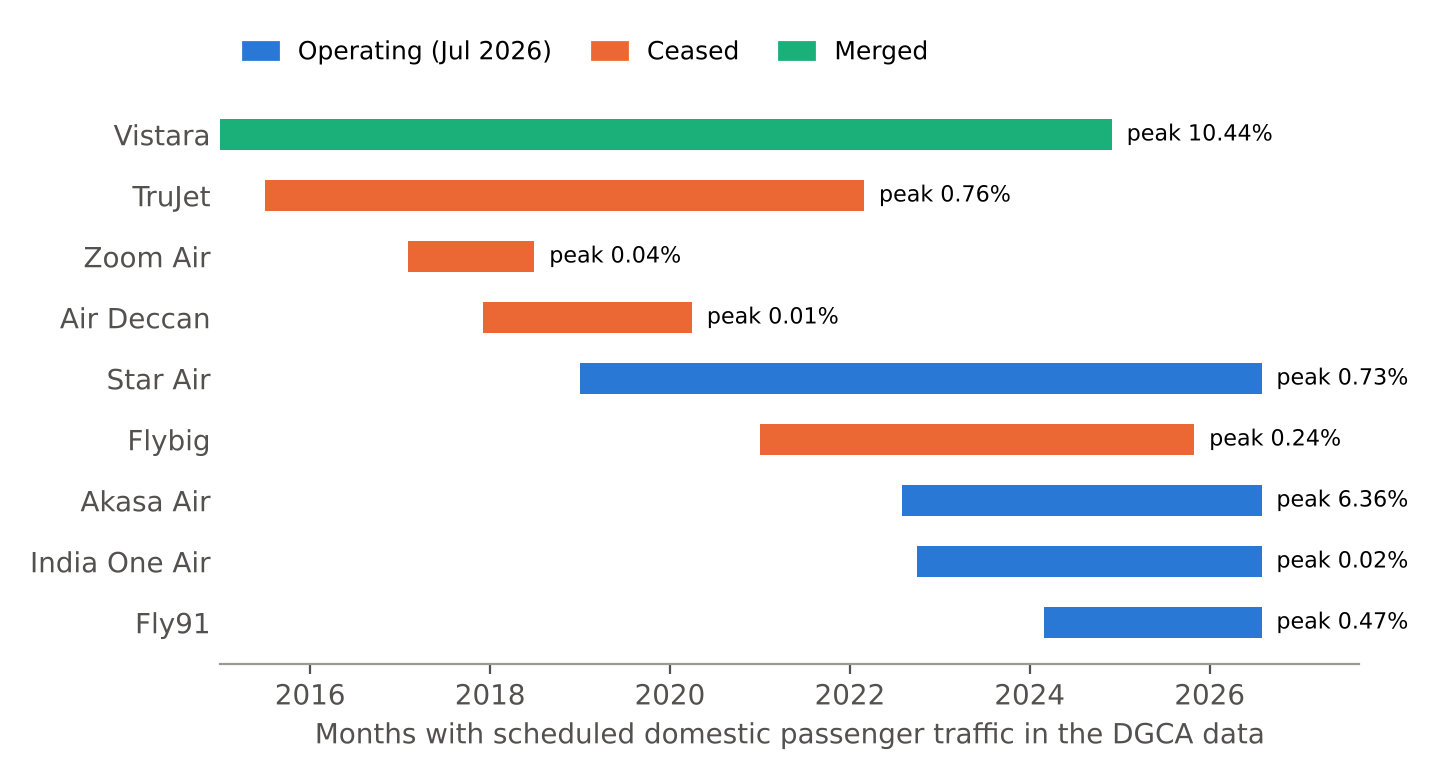
\includegraphics[width=0.92\textwidth]{figures/fig_o3_lifespans.png}
\captionof{figure}{O3: Operating span and peak passenger share of the nine entrants, January 2015--July 2026; colour shows the outcome at July 2026. Source: DGCA via Kubicek (2026); authors' calculations.}
\label{fig:o3-life}
\end{minipage}



\par
\begingroup
\flowtablestyle
\fontsize{10}{12}\selectfont
\begin{longtable}{|l|l|l|r|r|l|}
\caption{Entrant observation dates, early passenger shares and outcomes.}\label{tab:detail-o3-summary}\label{tab:o3-outcomes}\\
\hline
\textbf{Airline} & \textbf{First} & \textbf{Last} & \textbf{$\tau=12$ (\%)} & \textbf{$\tau=24$ (\%)} & \textbf{Outcome}\\
\hline
\endfirsthead
\multicolumn{6}{c}{Table~\thetable\ (continued)}\\
\hline
\textbf{Airline} & \textbf{First} & \textbf{Last} & \textbf{$\tau=12$ (\%)} & \textbf{$\tau=24$ (\%)} & \textbf{Outcome}\\
\hline
\endhead
\endfoot
\endlastfoot
Vistara & Jan 2015 & Nov 2024 & 1.97 & 3.27 & Merged\\
\hline
Akasa Air & Aug 2022 & Jul 2026 & 4.24 & 4.51 & Operating\\
\hline
TruJet & Jul 2015 & Feb 2022 & 0.35 & 0.48 & Ceased\\
\hline
Star Air & Jan 2019 & Jul 2026 & 0.09 & 0.20 & Operating\\
\hline
Fly91 & Mar 2024 & Jul 2026 & 0.08 & 0.23 & Operating\\
\hline
Flybig & Jan 2021 & Oct 2025 & 0.11 & 0.17 & Ceased\\
\hline
Zoom Air & Feb 2017 & Jun 2018 & 0.03 & -- & Ceased\\*
\noalign{\hrule height\arrayrulewidth\nobreak}
India One Air & Oct 2022 & Jul 2026 & 0.01 & 0.02 & Operating\\*
\noalign{\hrule height\arrayrulewidth\nobreak}
Air Deccan & Dec 2017 & Mar 2020 & -- & -- & Ceased\\*
\noalign{\hrule height\arrayrulewidth\nobreak}
\multicolumn{6}{@{}p{\linewidth}@{}}{\resultstablenotes{Traffic months count recorded observations. $\tau$ counts calendar months since first traffic. Dashes indicate no observation at that age. Peaks and 36-month shares are in Table~\ref{tab:o3-summary}.}{DGCA via Kubicek (2026); outcome sources below.}}\\
\end{longtable}
\endgroup

\begin{minipage}{\textwidth}
\centering
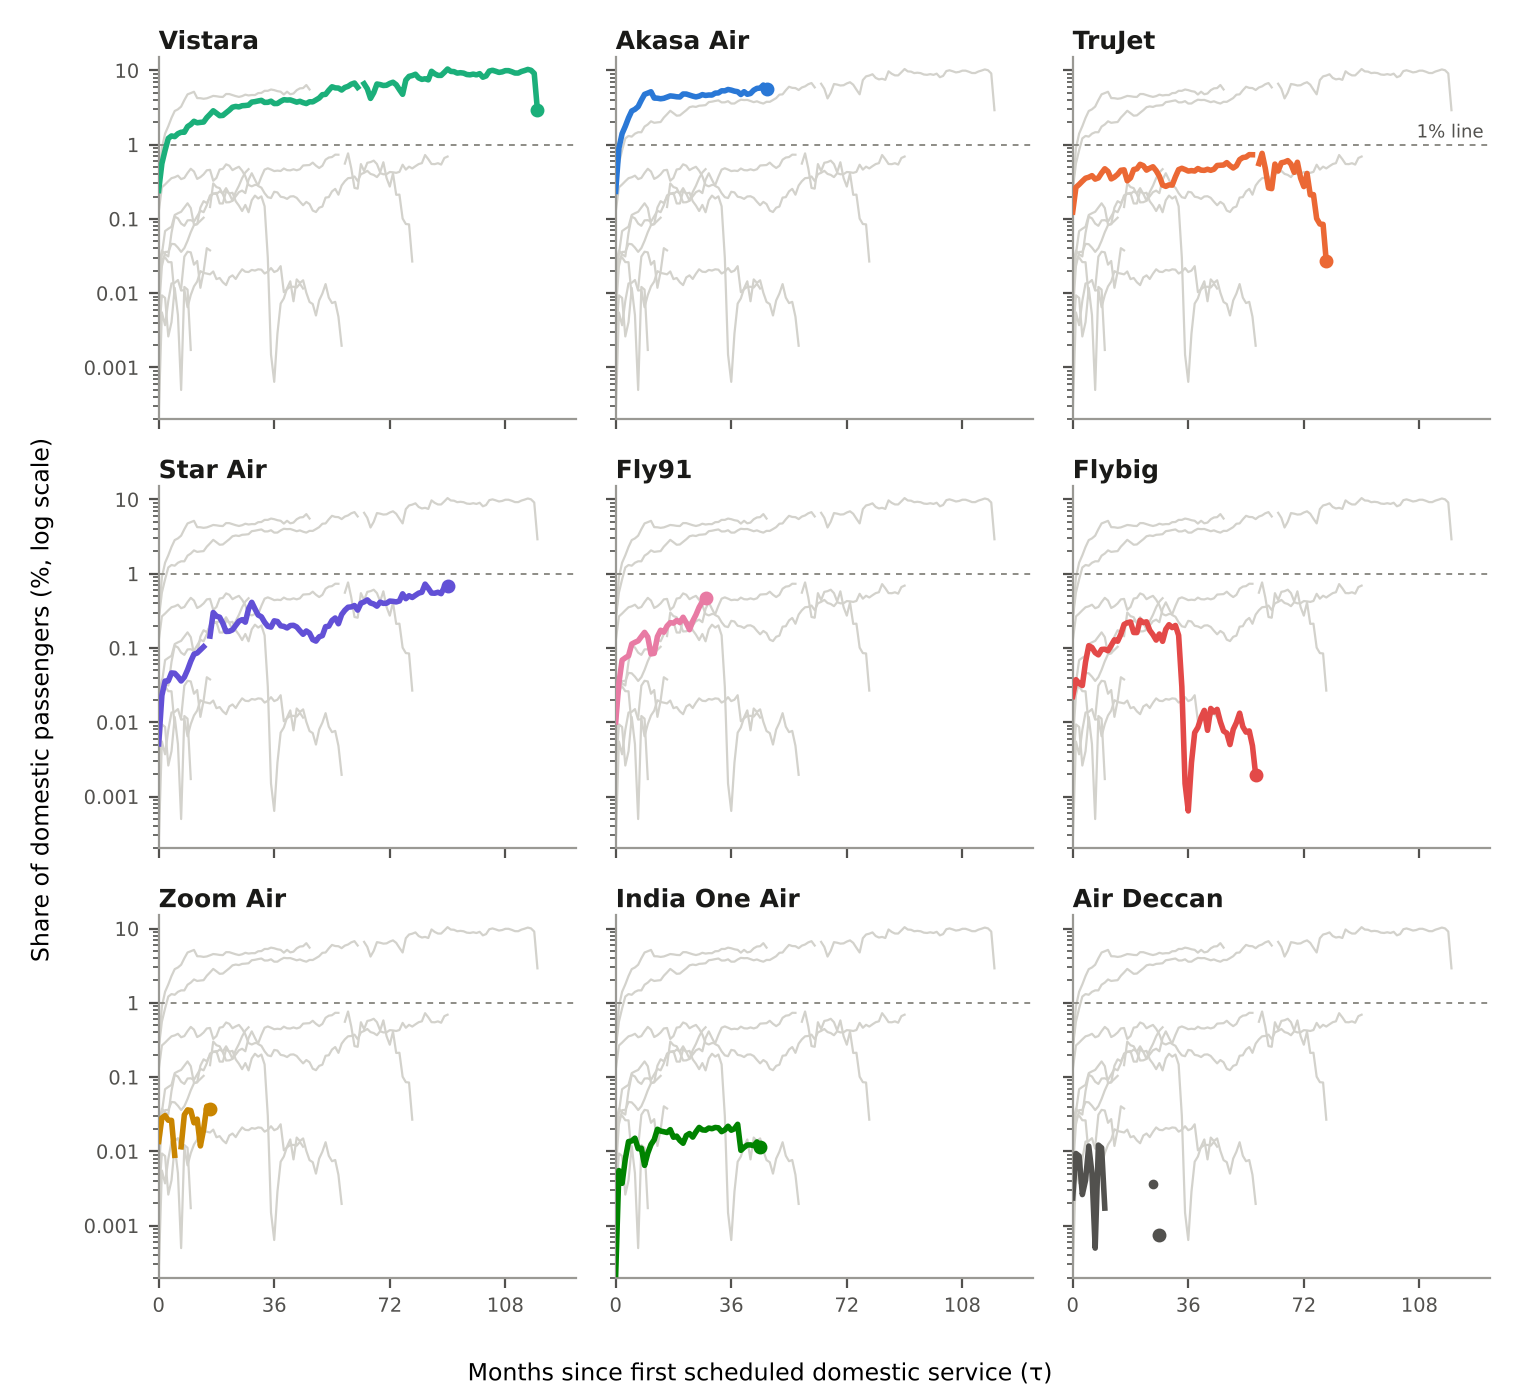
\includegraphics[width=0.82\textwidth]{figures/fig_o3_age.png}
\captionof{figure}{O3: Passenger share of the nine entrants by months since first service (log scale). One panel per entrant (coloured); the other eight are shown in grey for reference, and the dashed line marks 1\%. Each line ends at the airline's last observed month; gaps are months missing from the data (April 2020 for Vistara, TruJet and Star Air). Shares below 0.0002\% are drawn at the axis floor, and Vistara's last point (November 2024) is a partial month. Source: DGCA via Kubicek (2026); authors' calculations.}
\label{fig:o3-age}
\end{minipage}

\textbf{Sample exclusions.} Air Pegasus, Air Carnival, Air Odisha, Air Heritage, Pawan Hans and Air Taxi are excluded. AIX Connect is a rebrand, not a new entrant.

\textbf{Status records.} Vistara merged on 12 November 2024. SIA held 49\% of Vistara and 25.1\% of enlarged Air India \parencite{sia2025rule706a,tata2024vistaramerger}. Akasa began on 7 August 2022 \parencite{akasa2025anniversary}. Star Air, Fly91 and India One Air appear on the Ministry's operator list at 31 December 2024 \parencite[Section~1.7]{moca2025annual}.

TruJet closed on 11 May 2022 after lessor withdrawal. Its announced 2025 revival still required permit renewal and has no later traffic here \parencite{moca2026competition,seatrade2025trujet}. Flybig's deregistration request was in November 2025 and its AOC closed on 13 December 2025 \parencite{joshi2025flybig,moca2026competition}. Zoom suspended in July 2018 \parencite{businesstoday2019udan}. Air Deccan is on the Ministry's ceased-operator list \parencite{moca2024regional}. Traffic endpoints in Table~\ref{tab:detail-o3-summary} are distinct from legal closure dates.

\subsubsection{Seasonal route calculations}
\begingroup
\renewcommand{\theHequation}{review-o3-season-departures}
\textbf{Full-season counts.} Sum deduplicated services across both directions, counting only valid dates and operating weekdays within the chosen season:
\begin{equation}
D_{a,r,s}=\sum_{j\in(a,r)}\ \sum_{d\in s}
\mathbf{1}\{b_j\leq d\leq e_j\}\,
\mathbf{1}\{\mathrm{weekday}(d)\in W_j\}.
\tag{O3.1}\label{eq:o3-season-departures}
\end{equation}
Here $a,r,s$ denote airline, pair and season; $b_j,e_j,W_j$ are service $j$'s validity dates and weekdays. These are scheduled departures, not verified operations.
\renewcommand{\theHequation}{review-o3-season-share}
\begin{equation}
\mathrm{SeasonShare}_{a,r,s}=100\,
\frac{D_{a,r,s}}{\sum_b D_{b,r,s}}.
\tag{O3.2}\label{eq:o3-season-share}
\end{equation}
The denominator includes all recorded airlines on the airport pair in that season. Sole-operator records give $100(75/109)=68.8\%$ for regional entrants and $100(32/50)=64.0\%$ for ceased entrants. These are airline--airport-pair--season records.
\endgroup
\par


\par
\begingroup
\flowtablestyle
\fontsize{10}{12}\selectfont
\begin{longtable}{|>{\raggedright\arraybackslash}p{\dimexpr0.2\linewidth-2\tabcolsep-1.2\arrayrulewidth\relax}|>{\raggedright\arraybackslash}p{\dimexpr0.21\linewidth-2\tabcolsep-1.2\arrayrulewidth\relax}|>{\raggedright\arraybackslash}p{\dimexpr0.2\linewidth-2\tabcolsep-1.2\arrayrulewidth\relax}|>{\raggedright\arraybackslash}p{\dimexpr0.2\linewidth-2\tabcolsep-1.2\arrayrulewidth\relax}|>{\raggedright\arraybackslash}p{\dimexpr0.19\linewidth-2\tabcolsep-1.2\arrayrulewidth\relax}|}
\caption{Additional inputs for the full-season route comparisons.}\label{tab:o3-routes}\\
\hline
\textbf{Airline} & \textbf{Season} & \textbf{Scheduled departures} & \textbf{Median route share (\%)} & \textbf{Airlines with filings}\\
\hline
\endfirsthead
\multicolumn{5}{c}{Table~\thetable\ (continued)}\\
\hline
\textbf{Airline} & \textbf{Season} & \textbf{Scheduled departures} & \textbf{Median route share (\%)} & \textbf{Airlines with filings}\\
\hline
\endhead
\endfoot
\endlastfoot
Vistara & Winter 2023 & 43,523 & 20.3 & 9\\
\hline
Akasa Air & Summer 2026 & 32,340 & 22.8 & 9\\
\hline
TruJet & Winter 2021 & 9,463 & 100.0 & 10\\
\hline
Star Air & Summer 2026 & 11,589 & 100.0 & 9\\
\hline
Fly91 & Summer 2026 & 7,503 & 100.0 & 9\\
\hline
Flybig & Summer 2022 & 4,894 & 100.0 & 9\\
\hline
Zoom Air & Winter 2017 & 588 & 66.7 & 11\\
\hline
India One Air & Summer 2026 & 3,777 & 100.0 & 9\\
\hline
Air Deccan & Winter 2019 & 1,188 & 100.0 & 11\\*
\noalign{\hrule height\arrayrulewidth\nobreak}
\multicolumn{5}{@{}p{\linewidth}@{}}{\resultstablenotes{Median shares are across each entrant's airport pairs. The final column counts airlines with recorded filings in its selected season. Main counts are in Table~\ref{tab:results-o3-route-summary}.}{DGCA approved domestic schedules; authors' calculations.}}\\
\end{longtable}
\endgroup


\textbf{Separate monthly check.} TruJet met the 50\% threshold on 17 of 22 screened airport pairs in November 2019. In that month, TruJet supplied all 60 recorded scheduled flights on Chennai--Salem, giving a 100\% frequency share and HHI of 10,000. The airport pair carried 3,281 passengers across all airlines, while TruJet's national passenger share was 0.63\%. This monthly example is separate from the seasonal totals.

\Needspace{8\baselineskip}

\subsubsection{Financial inputs and worked ratios}
\label{app:eda-financial-coverage}


\par
\begingroup
\flowtablestyle
\fontsize{10}{12}\selectfont
\begin{longtable}{|>{\raggedright\arraybackslash}p{\dimexpr0.26\linewidth-2\tabcolsep-1.3333333333333333\arrayrulewidth\relax}|>{\raggedright\arraybackslash}p{\dimexpr0.37\linewidth-2\tabcolsep-1.3333333333333333\arrayrulewidth\relax}|>{\raggedright\arraybackslash}p{\dimexpr0.37\linewidth-2\tabcolsep-1.3333333333333333\arrayrulewidth\relax}|}
\caption{Revenue, profit and funding inputs for Vistara and Akasa Air.}\label{tab:detail-o3-fin}\\
\hline
\textbf{Input} & \textbf{Vistara (FY2023$\to$FY2024)} & \textbf{Akasa Air (FY2025$\to$FY2026)}\\
\hline
\endfirsthead
\multicolumn{3}{c}{Table~\thetable\ (continued)}\\
\hline
\textbf{Input} & \textbf{Vistara (FY2023$\to$FY2024)} & \textbf{Akasa Air (FY2025$\to$FY2026)}\\
\hline
\endhead
\endfoot
\endlastfoot
Operating income (Rs crore) & 12,261.4 $\to$ 15,310.3 & 4,582.7 $\to$ 6,167.9\\
\hline
Profit after tax (Rs crore) & $-1{,}393.3\to-581.1$ & $-1{,}983.5\to-2{,}716.0$\\
\hline
Funding & Rs~10,020 crore from Tata and Singapore Airlines by Aug 2024 & Equity round completed 19 Aug 2025; about US\$125 million is a press estimate\\*
\noalign{\hrule height\arrayrulewidth\nobreak}
\multicolumn{3}{@{}p{\linewidth}@{}}{\resultstablenotes{Revenue and PAT are in Rs crore and include domestic and international operations. Funding retains its reported currency. US\$125 million is a press estimate.}{\textcite{icra2024vistara,icra2026akasa}, Tata and Singapore Airlines company records, and \textcite{businessstandard2025akasa,akasa2025investment}.}}\\
\end{longtable}
\endgroup



For Vistara, the figures above give
\begin{align*}
\mathrm{Revenue\ growth}
&=100\frac{15{,}310.3-12{,}261.4}{12{,}261.4}\approx24.87\%,\\
\mathrm{FY2024\ net\ margin}
&=100\frac{-581.1}{15{,}310.3}\approx-3.80\%.
\end{align*}
The same calculations give Akasa Air's revenue growth and net margins in Table~\ref{tab:o3-fin}.




\par\begingroup
\flowtablestyle
\fontsize{10}{12}\selectfont
\renewcommand{\arraystretch}{1.15}
\captionsetup[longtable]{font={small,color=authorSweta}}
\begin{longtable}{|>{\raggedright\arraybackslash}p{\dimexpr0.12\linewidth-2\tabcolsep-1.1666666666666667\arrayrulewidth\relax}|>{\raggedright\arraybackslash}p{\dimexpr0.15\linewidth-2\tabcolsep-1.1666666666666667\arrayrulewidth\relax}|>{\raggedright\arraybackslash}p{\dimexpr0.15\linewidth-2\tabcolsep-1.1666666666666667\arrayrulewidth\relax}|>{\raggedright\arraybackslash}p{\dimexpr0.12\linewidth-2\tabcolsep-1.1666666666666667\arrayrulewidth\relax}|>{\raggedright\arraybackslash}p{\dimexpr0.15\linewidth-2\tabcolsep-1.1666666666666667\arrayrulewidth\relax}|>{\raggedright\arraybackslash}p{\dimexpr0.31\linewidth-2\tabcolsep-1.1666666666666667\arrayrulewidth\relax}|}
\caption{O3: Public financial evidence for the seven regional entrants (Rs crore).}\label{tab:o3-fy25}\\
\hline
\textbf{Airline (outcome)} & \textbf{Year} & \textbf{Result} & \textbf{Revenue} & \textbf{Result / revenue (\%)} & \textbf{Basis} \\
\hline
\endfirsthead
\multicolumn{6}{c}{Table~\thetable\ (continued)}\\
\hline
\textbf{Airline (outcome)} & \textbf{Year} & \textbf{Result} & \textbf{Revenue} & \textbf{Result / revenue (\%)} & \textbf{Basis} \\
\hline
\endhead
\endfoot
\endlastfoot

Fly91 (operating) & FY2024; FY2025 & $-31.42$; $-67.65$ & n.a.; 127.4 & n.a.; $-53.1$ & Ministry, after tax, FY2025 provisional; revenue press-reported \\
\hline
Star Air (operating) & FY2023; FY2024; FY2025 & $-20.84$; $-33.31$; $+68.75$ & n.a.; about 360; about 650 & n.a.; about $-9$; about $+11$ & Ministry, after tax, FY2025 provisional; revenue management-reported \\
\hline
India One Air (operating) & FY2023; FY2024; FY2025 & $-8.73$; $-3.23$; $+3.34$ & n.a. & n.a. & Ministry, after tax, FY2025 provisional \\
\hline
Flybig (ceased) & FY2023; FY2024 & $+5.59$; $+4.83$ & n.a. & n.a. & Ministry, after tax; no FY2025 figure \\
\hline
TruJet (ceased) & FY2017, FY2018, FY2019 & $-80.77$; $-85.15$; $-41.00$ & 126.14; 195.68; 265.00 & $-64.0$; $-43.5$; $-15.5$ & Operating result \parencite{rajyasabha2019finances}; FY2019 provisional \\
\hline
TruJet & FY2019, FY2020, FY2021 & $-17.56$; $-10.17$; $-143.16$ & n.a. & n.a. & Operating result \parencite{rajyasabha2021finances}; FY2020--21 provisional \\
\hline
Zoom Air (ceased) & FY2017, FY2018, FY2019 & $+0.14$; $+0.81$; $-1.40$ & 2.61; 17.40; 10.36 & $+5.4$; $+4.7$; $-13.5$ & Operating result \parencite{rajyasabha2019finances}; FY2019 provisional \\
\hline
Air Deccan (ceased) & FY2018, FY2019 & $-13.55$; $-28.90$ & 62.93; 4.70 & $-21.5$; n.m. & Operating result \parencite{rajyasabha2019finances}; may include non-scheduled business \\*
\noalign{\hrule height\arrayrulewidth\nobreak}

\multicolumn{6}{@{}p{\linewidth}@{}}{\footnotesize\raggedright ``n.a.'' means unavailable. ``n.m.'' means not meaningful. Ministry figures are after income taxes and extraordinary items. Operating results exclude interest, tax and other non-operating items. TruJet's FY2019 figures show the provisional 2019 reply and its 2021 revision. Fly91 and Star Air revenues are press-reported, without inspection of the filings. Different accounting bases are not pooled. Sources: \textcite{moca2025losses}; \textcite{rajyasabha2019finances,rajyasabha2021finances}; \textcite{whalesbook2026fly91}; \textcite{aviationa2z2026star}.}\\
\end{longtable}
\endgroup\par\medskip

\end{mergedcontribution}

\subsection{O4: Route coverage, sensitivity and unused capacity}
\label{app:o4-route-preparation}
\begin{mergedcontribution}{authorGoutham}
The focus-period CSV also retains IndiGo minus Air India Group share. This signed measure can be negative and differs from the nonnegative leader--rival gap in Appendix~\ref{app:shared-calculations}.

\subsubsection{Route inputs and screening}
\label{app:eda-route-support}
Table~\ref{tab:review-route-samples} separates overlapping samples from recovered DGCA schedules. Directions are pooled; O3 uses brands, O4 ownership groups. Counts with different units are not added.

\begin{resultstable}{Samples drawn from the DGCA schedule archive.}{tab:review-route-samples}
\color{black}
\begin{tabular}{|>{\raggedright\arraybackslash}p{\dimexpr0.31\linewidth-2\tabcolsep-1.5\arrayrulewidth\relax}|>{\raggedright\arraybackslash}p{\dimexpr0.69\linewidth-2\tabcolsep-1.5\arrayrulewidth\relax}|}
\hline
\textbf{Sample} & \textbf{Coverage and observation unit} \\
\hline
Entrant full-season & Nine entrants; 229 airline--pair--season observations; all scheduled departures in each selected season \\
\hline
Entrant major routes & 20 pairs, April 2019--July 2026; airline--pair--month \\
\hline
TruJet regional extension & 30 pairs, 14 observed months in 2019--2022; airline--pair--month \\
\hline
Ownership concentration & 20 fixed pairs; 1,150 pair--months across 66 available months, April 2019--September 2026 \\
\hline
\end{tabular}
\par\vspace{5pt}{\footnotesize\setstretch{1.05}\raggedright \textbf{Note:} Entrants use the latest usable season before closure/merger or latest available season. O4's fixed top 20 and nested top ten use 2025 passenger totals.\par\textbf{Source:} Sweta\textquotesingle s and Goutham\textquotesingle s DGCA schedule preparation.\par}
\end{resultstable}
 Of 228 schedule PDFs, 92 supply retained departure data. Valid services are expanded by operating day, deduplicated by flight/date/direction and pooled across directions. PDF, page and row references are preserved.

Retain full months with at least ten airport pairs and endpoint discrepancy
\[
100\frac{\sum_a|D_a-A_a|}{\sum_aD_a}\leq5\%,
\]
where $D_a,A_a$ are airline $a$'s departures and arrivals across both directions. Excluding Chennai--Hyderabad in February--March 2022, where TruJet's plan extends beyond suspension, gives $1{,}152-2=1{,}150$ observations. Exactly 303 satisfy $D_a=A_a$ for every airline. Missing filings can still pass this screen.

\subsubsection{Route calculations and sensitivity}
\label{app:o4-flags}
Apply H5 and H6 from Section~\ref{sec:hypotheses} \parencite[Section~2.1]{dojftc2023merger}. IndiGo exposure is study-defined at 60\%, and sole operation requires 100\%. Joint conditions are in Table~\ref{tab:o4-route-focus}.

A tie for second prevents a unique leading pair. Exactly two groups tied for first still form a unique pair, but neither leads uniquely. Alphabetical ordering is for display only. Missing observations are excluded and observed zeros retained.

Figure~\ref{fig:o4-route-heatmap} uses a common 0--10,000 scale; grey cells are missing, not interpolated.

\begin{figure}[H]
\centering
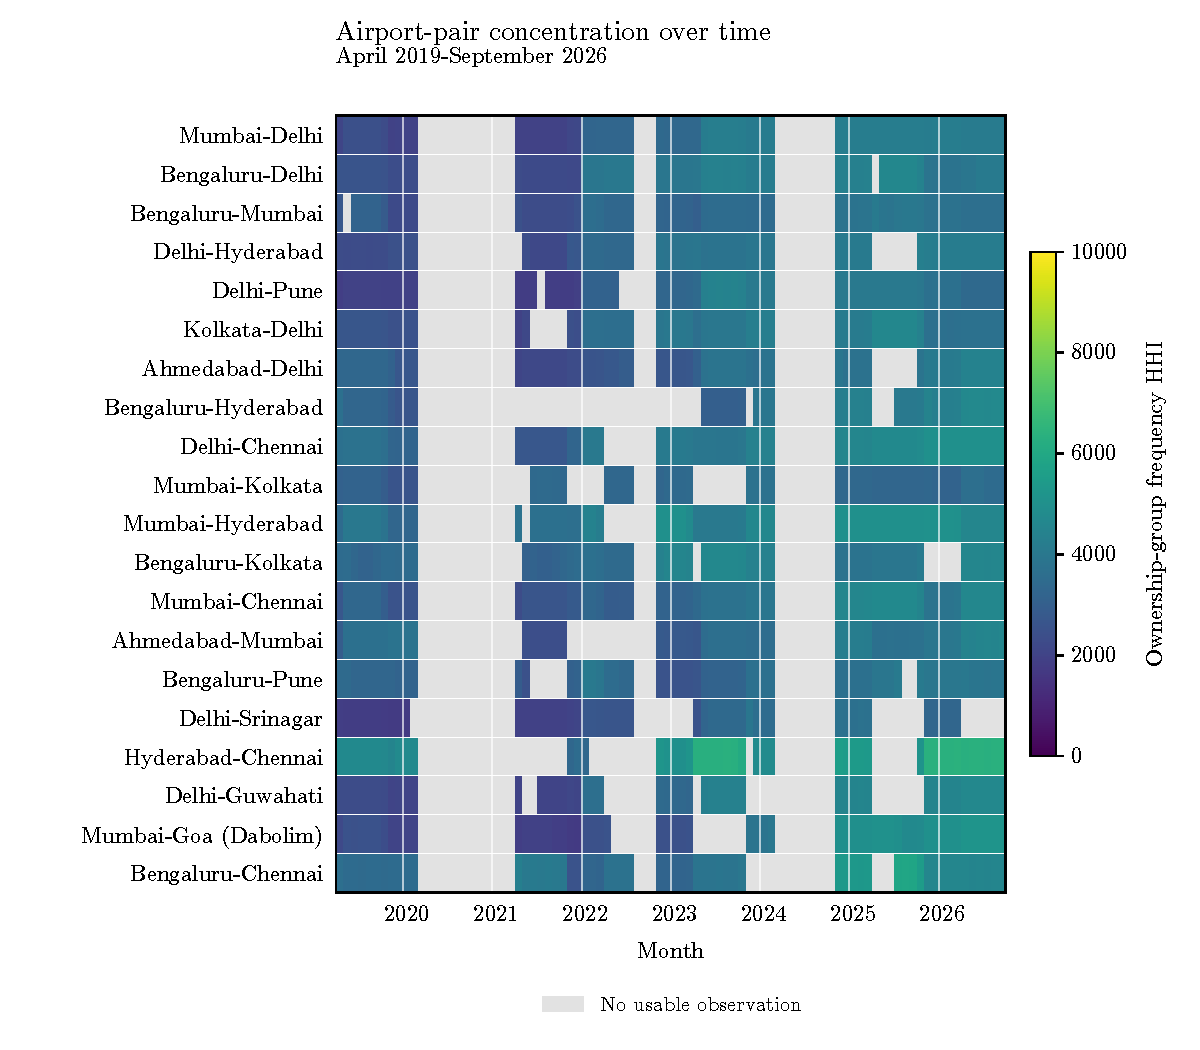
\includegraphics[width=\linewidth]{figures/o4_route_hhi_heatmap.pdf}
\caption{Ownership-group frequency HHI by airport pair and month.}
\label{fig:o4-route-heatmap}
\vspace{2pt}
\begin{minipage}{\linewidth}
\footnotesize\setstretch{1.1}
\textit{Source:} DGCA approved domestic schedules; authors' calculations.
\end{minipage}
\end{figure}


\label{app:o4-route-calculations}
\textbf{Delhi--Pune, June 2026.} Prepared DGCA schedules give Air India Group $618=472+146$ flights, IndiGo 524, SpiceJet 168 and Akasa 120, totalling 1,430. Applying Appendix~\ref{app:shared-calculations} without rounding intermediate shares,
\[
\begin{aligned}
\HHI&=10{,}000\frac{618^2+524^2+168^2+120^2}{1{,}430^2}\approx3{,}418.87,\\
\mathrm{CR2}&=100\frac{618+524}{1{,}430}\approx79.8601\%.
\end{aligned}
\]
\[
\begin{aligned}
\mathrm{Gap}&=100(618-524)/1{,}430\approx6.5734\ \mathrm{pp},\\
\mathrm{Fringe}&=100-\mathrm{CR2}\approx20.1399\%,\qquad
s_I=100(524/1{,}430)\approx36.6434\%.
\end{aligned}
\]
HHI exceeds 1,800, while CR2 and the share gap are below the joint-condition thresholds.

\Needspace{4\baselineskip}

\label{app:o4-route-checks}
Additional condition percentages are
\[
\begin{aligned}
\mathrm{CR2}\geq80\% &: 100(583/1{,}150)=50.70\%,\\
\mathrm{Gap}>20\ \mathrm{pp} &: 100(368/1{,}150)=32.00\%,\\
\mathrm{Second\mbox{-}place\ tie} &: 100(58/1{,}150)=5.04\%.
\end{aligned}
\]
Conditions overlap. The leading-pair count is in Table~\ref{tab:o4-route-results}.

Full-period medians are CR2 80.00\%, gap 13.73 pp, fringe 20.00\% and IndiGo frequency share 43.60\%. The 79 observations meeting the IndiGo $\geq60\%$ flag occur on Bengaluru--Kolkata, Chennai--Hyderabad and Bengaluru--Chennai. Monthly exposure ranges from 0\% to 11.11\% of available airport pairs. In December 2025, Chennai--Hyderabad is the only one of 19 available airport pairs meeting the flag, with IndiGo at 78.10\%.

Table~\ref{tab:o4-route-sensitivity} compares overlapping subsets, not additive samples. Exact endpoint agreement does not prove complete airline filings.

\begin{minipage}{\linewidth}
\captionsetup{font=small,labelfont=bf,justification=raggedright,singlelinecheck=false,hypcap=false}
\captionof{table}{Route concentration and IndiGo exposure across sample definitions.}
\label{tab:o4-route-sensitivity}
\centering
{\small\setstretch{1.1}\setlength{\tabcolsep}{4pt}\fontsize{10}{12}\selectfont\setstretch{1}\setlength{\tabcolsep}{3pt}
\renewcommand{\arraystretch}{1.15}
\begin{tabular}{|>{\raggedright\arraybackslash}p{\dimexpr0.4\linewidth-2\tabcolsep-1.25\arrayrulewidth\relax}|>{\raggedright\arraybackslash}p{\dimexpr0.2\linewidth-2\tabcolsep-1.25\arrayrulewidth\relax}|>{\raggedright\arraybackslash}p{\dimexpr0.2\linewidth-2\tabcolsep-1.25\arrayrulewidth\relax}|>{\raggedright\arraybackslash}p{\dimexpr0.2\linewidth-2\tabcolsep-1.25\arrayrulewidth\relax}|}
\hline
\textbf{Sample} & \textbf{$N$} & \textbf{HHI $>1{,}800$: $n$ (\%)} & \textbf{IndiGo $\geq60\%$: $n$ (\%)} \\
\hline
Full sample & 1,150 & 1,143 (99.39\%) & 79 (6.87\%) \\
\hline
Exact endpoint matches & 303 & 301 (99.34\%) & 26 (8.58\%) \\
\hline
December 2025 & 19 & 19 (100.00\%) & 1 (5.26\%) \\
\hline
\end{tabular}
\par}
\vspace{4pt}
{\footnotesize\setstretch{1.1}\raggedright\textit{Note:} $N$ is retained airport-pair/month observations and $n$ is observations meeting each condition. Exact matches and December 2025 are subsets of April 2019--September 2026. No subset contains an IndiGo-only observation.\par
\textit{Source:} DGCA approved domestic schedules; authors' calculations.\par}
\end{minipage}

\subsubsection{National and focus-period checks}
\label{app:o4-national-summary}
The national condition counts are in Table~\ref{tab:o4-national-results}. HHI exceeds 1,800 in all 138 observed months. Focus-period HHI ranges from 4,468.57 to 5,144.35 and fringe share from 8.30\% to 10.87\%. The bound stated with H5 follows from $s_1^2+s_2^2\geq(s_1+s_2)^2/2$.

The second-largest group is Jet (January 2015--January 2019), SpiceJet (February 2019--April 2021), Air India (May--August 2021), Vistara (September 2021), Go First (October--December 2021) and Air India Group (January 2022 onward), using the passenger series in Figure~\ref{fig:o4-national-eda}.


\label{app:o4-route-focus}
Table~\ref{tab:o4-route-focus} gives the retained and possible observations. Monthly coverage ranges from 6--10 airport pairs for the top ten and 12--20 for the top 20. Both are complete through March 2025, lowest in April (6/12), and 10/19 from November 2025 onward.

Route medians use retained airport-pair/month observations, without passenger or flight weighting. National medians use the 20 monthly observations.

The joint counts in Table~\ref{tab:o4-route-focus} give $100(9/184)=4.89\%$ for the top ten and $100(50/350)=14.29\%$ for the top 20.
First-place ties are counted separately: IndiGo leads in 86, Air India in 94 and both tie in four top-10 observations; the corresponding top-20 counts are 214, 132 and four. IndiGo supplies at least 60\% of scheduled flights in 26 of 350 top-20 observations and none of the 184 top-ten observations. Neither focus-period sample contains an IndiGo-only observation.

\subsubsection{Capacity-buffer calculation}
\label{app:o4-capacity-buffer}
Let $I$ denote IndiGo and $j$ a retained rival airline brand. For month $t$, unused rival capacity $U_t$ and the buffer percentage $B_t$ are
\[
U_t=\sum_{j\ne I}(\mathrm{ASK}_{jt}-\mathrm{RPK}_{jt}),
\qquad B_t=100\frac{U_t}{\mathrm{RPK}_{It}}.
\]
Each rival brand is counted once. The denominator is all IndiGo RPK. The worked inputs and results are in Table~\ref{tab:o4-capacity-inputs}.

\begin{minipage}{\linewidth}
\captionsetup{font=small,labelfont=bf,justification=raggedright,singlelinecheck=false,hypcap=false}
\captionof{table}{Capacity-buffer inputs and calculation, December 2024 and December 2025.}
\label{tab:o4-capacity-inputs}
\centering
{\fontsize{10}{12}\selectfont\setstretch{1}\setlength{\tabcolsep}{3pt}
\renewcommand{\arraystretch}{1.15}
\begin{tabular}{|>{\raggedright\arraybackslash}p{\dimexpr0.48\linewidth-2\tabcolsep-1.3333333333333333\arrayrulewidth\relax}|>{\raggedright\arraybackslash}p{\dimexpr0.26\linewidth-2\tabcolsep-1.3333333333333333\arrayrulewidth\relax}|>{\raggedright\arraybackslash}p{\dimexpr0.26\linewidth-2\tabcolsep-1.3333333333333333\arrayrulewidth\relax}|}
\hline
\textbf{Input / calculation} & \textbf{Dec 2024} & \textbf{Dec 2025} \\
\hline
Rivals' ASK & 6.384761131 & 6.618678370 \\
\hline
Rivals' RPK & 5.492545663 & 5.946741054 \\
\hline
IndiGo RPK & 9.113052 & 8.207875 \\
\hline
$U=$ rivals' ASK minus RPK & 0.892215468 & 0.671937316 \\
\hline
$B=100U/\mathrm{RPK}_{I}$ (\%) & 9.7905 & 8.1865 \\
\hline
\end{tabular}\par}
\vspace{4pt}
{\footnotesize\setstretch{1.0}\raggedright\textit{Note:} ASK, RPK and $U$ are in billions. Inputs retain precision for the calculation; source-unit conversion is in Appendix~\ref{app:shared-calculations}.\par
\textit{Source:} DGCA via Kubicek (2026); authors' calculations.\par}
\end{minipage}

For December 2025, $B=100(0.671937316)/8.207875\approx8.1865\%$. The change is $8.1865-9.7905=-1.6040$ pp. Unused rival capacity changes by $100(0.671937316/0.892215468-1)=-24.69\%$.

\textbf{Validity checks.} The 19 records cover ten brands in December 2024 and nine in December 2025, including IndiGo. All satisfy ASK $>0$ and $0\leq\mathrm{RPK}\leq\mathrm{ASK}$. Flybig has no retained positive-passenger record in December 2025. The historical zero-capacity records in Appendix~\ref{app:o1-cleaning} are excluded. Airline inputs are retained in the CSV.

\end{mergedcontribution}
\Needspace{24\baselineskip}
\section{Reproduction}
\label{app:reproduction}
\textbf{Code repository:} \url{https://github.com/Goutham7358/Assignment3_Code}

Use Python 3.11 or newer and install dependencies from the repository root with \texttt{python -m pip install -r requirements.txt}. Run the programs in Table~\ref{tab:appendix-code-map} from that directory. The \href{https://github.com/Goutham7358/Assignment3_Code/blob/main/README.md}{README} links commands to outputs. Report values may be rounded further than the CSV outputs.

\begin{resultstable}{Programs and outputs for reproducing the results.}{tab:appendix-code-map}
\begin{tabular}{|>{\raggedright\arraybackslash}p{\dimexpr0.09\linewidth-2\tabcolsep-1.3333333333333333\arrayrulewidth\relax}|>{\raggedright\arraybackslash}p{\dimexpr0.56\linewidth-2\tabcolsep-1.3333333333333333\arrayrulewidth\relax}|>{\raggedright\arraybackslash}p{\dimexpr0.35\linewidth-2\tabcolsep-1.3333333333333333\arrayrulewidth\relax}|}
\hline
\textbf{Obj.} & \textbf{Programs} & \textbf{Outputs / guide} \\
\hline
O1 & \path{O1/export_results_tables.py} & \path{O1/results/}, \path{O1/figures/}; \href{https://github.com/Goutham7358/Assignment3_Code/blob/main/O1/README.md}{O1 instructions} \\
\hline
O2 & \path{O2/run_analysis.py} & \path{O2/output/}; \href{https://github.com/Goutham7358/Assignment3_Code/blob/main/O2/README.md}{O2 instructions} \\
\hline
O3 & & \\
\hline
O4 & \path{O4/run_analysis.py} & \path{O4/output/}; \href{https://github.com/Goutham7358/Assignment3_Code/blob/main/O4/README.md}{O4 instructions} \\
\hline
\end{tabular}
\par\vspace{4pt}
{\footnotesize\raggedright\textbf{Source:} Authors\textquotesingle\ code repository.\par}
\end{resultstable}
